\begin{table}[h!]
    \centering
    \begin{tabular}{ |l|c|c|c|c|c| } 
        \hline
        metrics & run1 & run2 & run3 & run4 & run5 \\ \hline
        num\_q & 657 & 669 & 669 & 667 & 667 \\ \hline
        num\_ret & 646525 & 658446 & 658347 & 652222 & 657903 \\ \hline
        num\_rel & 2550 & 2611 & 2611 & 2603 & 2600 \\ \hline
        num\_rel\_ret & 1772 & 2182 & 2191 & 1866 & 2232 \\ \hline
        map & 0.1307 & 0.2022 & 0.2335 & 0.1856 & 0.2351 \\ \hline
        gm\_map & 0.0117 & 0.046 & 0.061 & 0.0239 & 0.0629 \\ \hline
        Rprec & 0.1041 & 0.1697 & 0.1989 & 0.1654 & 0.2022 \\ \hline
        bpref & 0.3142 & 0.3734 & 0.3869 & 0.3466 & 0.3861 \\ \hline
        recip\_rank & 0.2436 & 0.3287 & 0.3891 & 0.3441 & 0.3945 \\ \hline
        iprec\_at\_recall\_0.00 & 0.2553 & 0.3499 & 0.4134 & 0.3584 & 0.4182 \\ \hline
        iprec\_at\_recall\_0.20 & 0.2387 & 0.3324 & 0.3873 & 0.3353 & 0.3927 \\ \hline
        iprec\_at\_recall\_0.40 & 0.1441 & 0.2316 & 0.2732 & 0.2066 & 0.2716 \\ \hline
        iprec\_at\_recall\_0.60 & 0.0965 & 0.1786 & 0.1996 & 0.1388 & 0.2014 \\ \hline
        iprec\_at\_recall\_0.80 & 0.0628 & 0.1178 & 0.1311 & 0.0887 & 0.1295 \\ \hline
        iprec\_at\_recall\_1.00 & 0.0525 & 0.0954 & 0.1031 & 0.0704 & 0.1028 \\ \hline
        P\_10 & 0.0848 & 0.1296 & 0.1435 & 0.1126 & 0.1432 \\ \hline
        P\_100 & 0.0186 & 0.0256 & 0.0268 & 0.0222 & 0.0268 \\ \hline
        P\_1000 & 0.0027 & 0.0033 & 0.0033 & 0.0028 & 0.0033 \\ \hline
        recall\_10 & 0.2166 & 0.3352 & 0.367 & 0.2849 & 0.3621 \\ \hline
        recall\_100 & 0.4718 & 0.6426 & 0.6714 & 0.5536 & 0.6723 \\ \hline
        recall\_1000 & 0.6816 & 0.8192 & 0.8218 & 0.7004 & 0.8392 \\ \hline
        infAP & 0.1307 & 0.2022 & 0.2335 & 0.1856 & 0.2351 \\ \hline
        gm\_bpref & 0.0152 & 0.0387 & 0.0405 & 0.022 & 0.038 \\ \hline
        utility & -978.6621 & -977.701 & -977.5262 & -972.2489 & -979.6687 \\ \hline
        ndcg & 0.2719 & 0.3655 & 0.3924 & 0.3291 & 0.3982 \\ \hline
        ndcg\_rel & 0.236 & 0.3119 & 0.3416 & 0.2939 & 0.3471 \\ \hline
        Rndcg & 0.1708 & 0.2387 & 0.2657 & 0.2271 & 0.2714 \\ \hline
        ndcg\_cut\_5 & 0.1285 & 0.1908 & 0.2232 & 0.1854 & 0.2269 \\ \hline
        ndcg\_cut\_10 & 0.1609 & 0.2426 & 0.2739 & 0.2227 & 0.2758 \\ \hline
        ndcg\_cut\_100 & 0.2351 & 0.3349 & 0.3652 & 0.3016 & 0.3678 \\ \hline
        ndcg\_cut\_1000 & 0.2719 & 0.3655 & 0.3924 & 0.3291 & 0.3982 \\ \hline
        map\_cut\_10 & 0.1046 & 0.1665 & 0.1975 & 0.1556 & 0.1993 \\ \hline
        map\_cut\_100 & 0.1284 & 0.2 & 0.2315 & 0.1836 & 0.2328 \\ \hline
        map\_cut\_1000 & 0.1307 & 0.2022 & 0.2335 & 0.1856 & 0.2351 \\ \hline
        
    \end{tabular}
    \caption{English results from TREC eval}
    \label{table:results}
\end{table}
\pagebreak
\begin{itemize}
    \item \textbf{run1}: PorterStemFilter, Standard tokenizer, LenghtFilter between 2 and 15, "long-stoplist-fr.txt" for StopFilter, LowerCaseFilter, BM25Similarity;
    \item \textbf{run2}: FrenchLightStemFilter, Standard tokenizer, LenghtFilter between 2 and 15, "long-stoplist-fr.txt" for StopFilter, LowerCaseFilter, BM25Similarity;
    \item \textbf{run3}: FrenchLightStemFilter, Standard tokenizer, LenghtFilter between 2 and 15, "long-stoplist-fr.txt" for StopFilter, LowerCaseFilter,\\ BM25Similarity((float)1.2,(float)0.90);
    \item \textbf{run4}: PorterStemFilter, Standard tokenizer, LenghtFilter between 2 and 15, "long-stoplist.txt" for StopFilter, LowerCaseFilter, BM25Similarity((float)1.2,(float)0.90), EnglishPossessiveFilter;
    \item \textbf{run5}: FrenchLightStemFilter, Standard tokenizer, LenghtFilter between 2 and 15, "new-long-stoplist-fr.txt" for StopFilter, LowerCaseFilter,\\ BM25Similarity((float)1.2,(float)0.90), ElisionFilter with some common french articles and prepositions;
\end{itemize}




\begin{figure}[h!]
    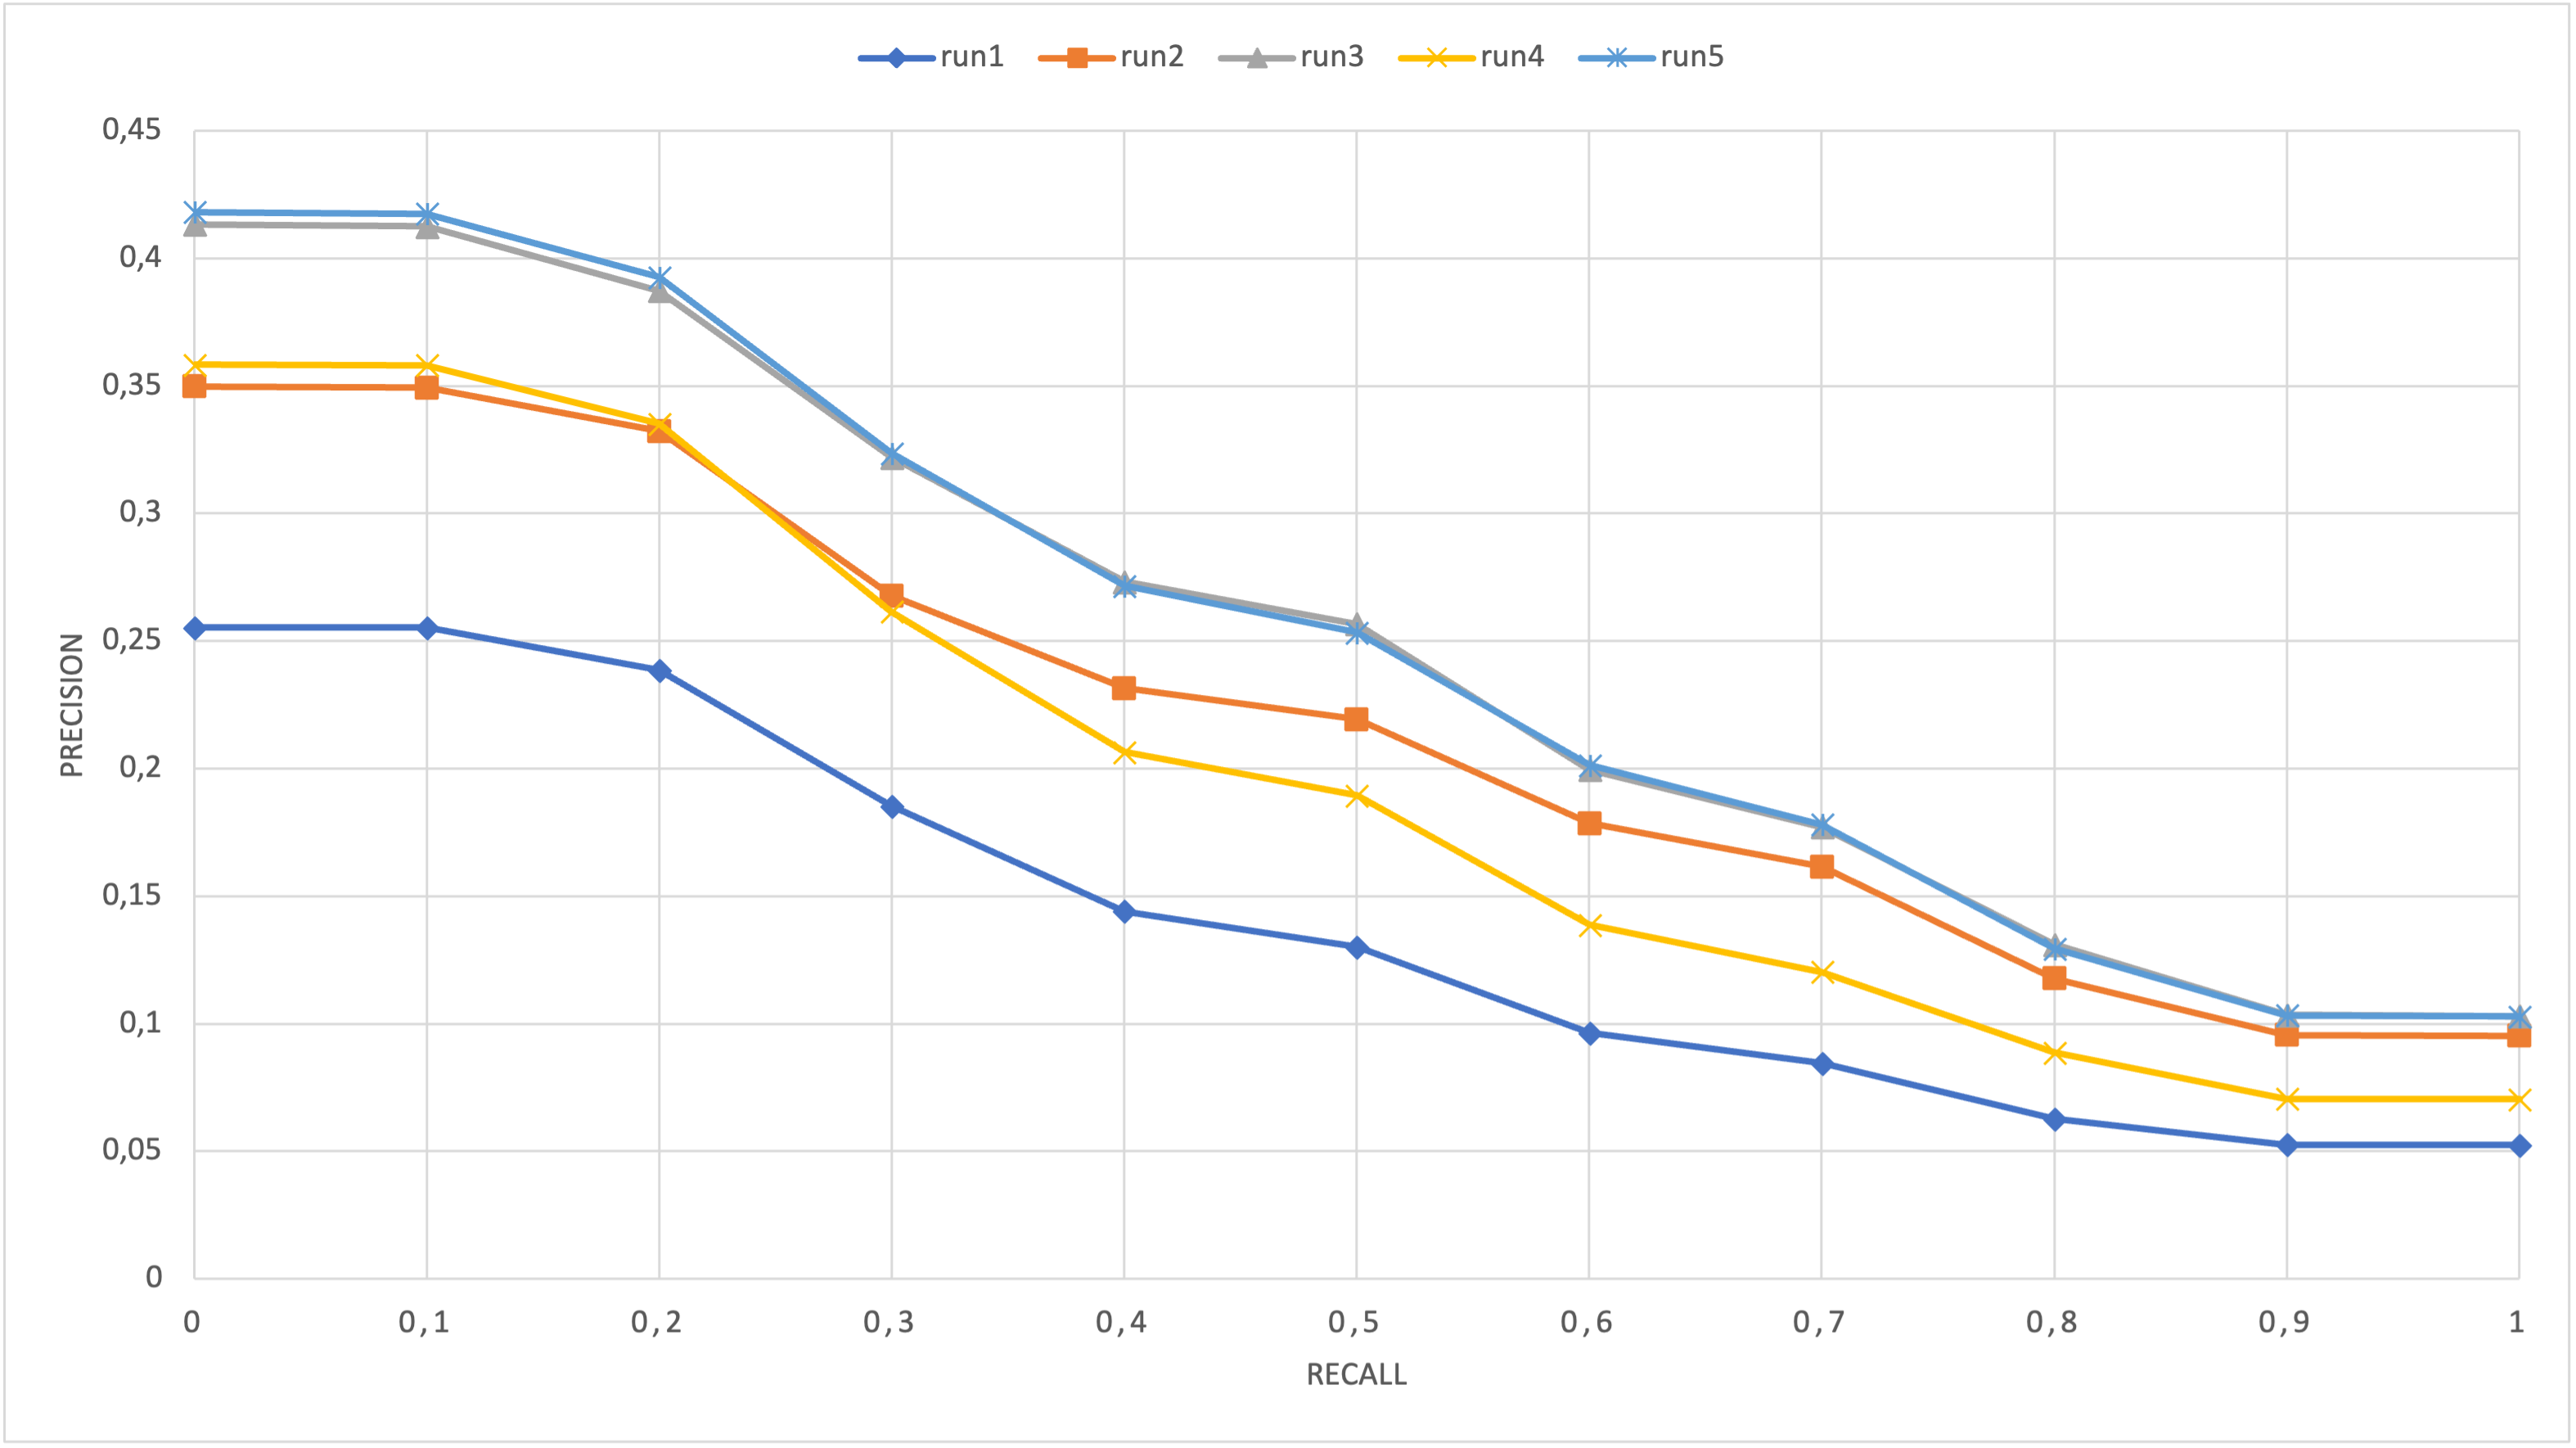
\includegraphics[width=\textwidth]{figure/PRgraph.png}
    \caption{Recall and precision graph}
    \label{fig:recallPrecision}
  \end{figure}